\subsubsection{\theoryC{Search for light pseudo-scalar with taus}}
\contributors{Giacomo Cacciapaglia, Gabriele Ferretti, Thomas Flacke, Hugo Serodio}\rt{There are comments to address.}

%\textbf{Authors: Giacomo Cacciapaglia$^a$, Gabriele Ferretti$^b$, Thomas Flacke$^c$ and Hugo Serodio$^d$}\\
%\textit{a) Universit\'{e} de Lyon, France; Universit\'{e} Lyon 1, Villeurbanne Cedex, France,
%b) Department of Physics, Chalmers University of Technology, Fysikg\aa rden, 41296 G\"oteborg, Sweden,
%c) Center for Theoretical Physics of the Universe, Institute for Basic Science (IBS), Daejeon, 34126, Korea,
%d) Department of Astronomy and Theoretical Physics, Lund University, SE-223 62 Lund, Sweden. }\\
%\texttt{g.cacciapaglia@ipnl.in2p3.fr, ferretti@chalmers.se, \\flacke@ibs.re.kr, hugo.serodio@thep.lu.se}


The discovered Higgs boson may be accompanied by additional light (pseudo-)scalars in models with an extended Higgs sector. We consider a pseudo-scalar singlets $\phi$, generically coupling as:
\begin{equation}
 {\mathcal{L}} \supset - \sum_\psi \frac{i C^\phi_\psi m_\psi \phi}{f_\phi} \bar \psi \gamma^5 \psi
+ \frac{\phi}{16\pi^2 f_\phi}\bigg(K^\phi_{G}\, G\tilde G + K^\phi_W\,  W \tilde{W} +K^\phi_B\, B \tilde B\bigg)\,, \label{eq:lagrTCP}
\end{equation}
where $f_\phi$ is a ``decay constant'' and $\psi$ labels the Standard Model fermions.
We focus on models of composite Higgs with partial compositeness described in terms of confining hyper-quarks~\cite{Ferretti:2013kya}. A universal feature of all these models is the presence of two such pseudo-scalars ($\phi= a, \,\eta'$), whose couplings  in \eq{eq:lagrTCP} can be computed from the underlying model.  Additional couplings, including the higher dimensional couplings to the Higgs boson, not included in \eq{eq:lagrTCP}, are also determined by the underlying theory (see \citeref{Belyaev:2016ftv} for details). In \citeref{Belyaev:2016ftv} we narrowed down this class of models to a total of twelve, providing possible benchmarks in the search of new physics. 

\begin{figure*}[t] 
\begin{center}
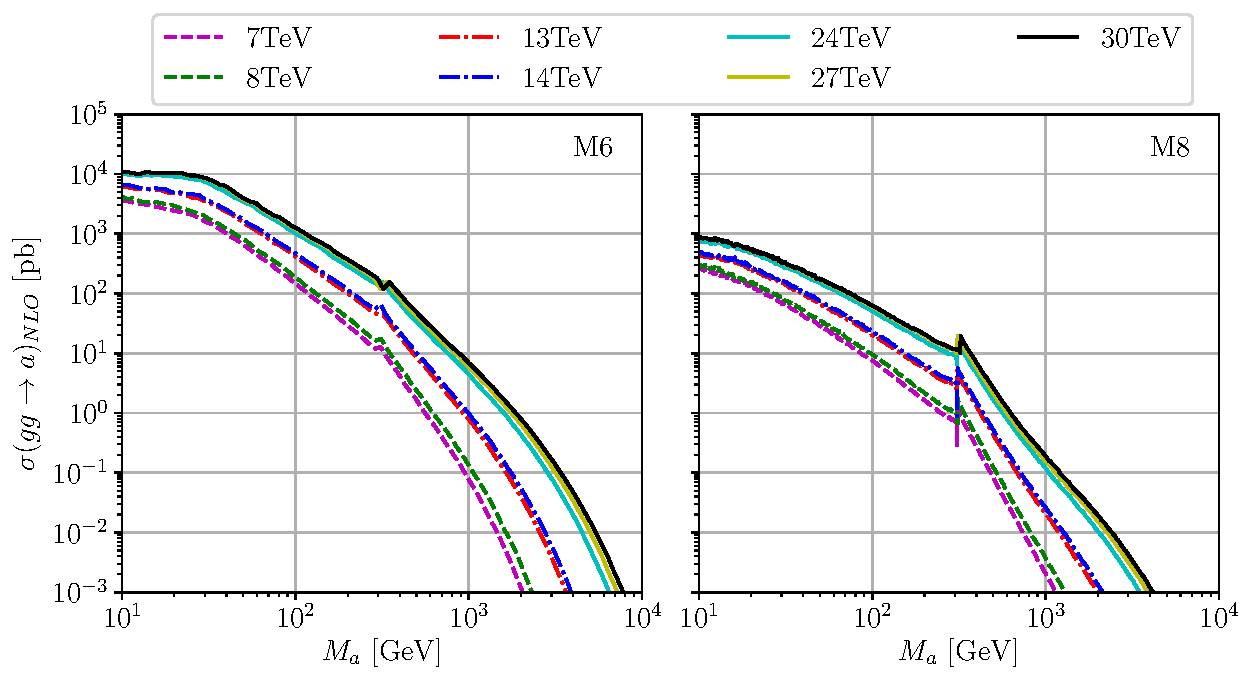
\includegraphics[width=0.99\textwidth]{\main/section7OtherSignatures/img/Fig1_TimidPNGB.pdf} 
\end{center}
\caption{\label{fig:Fig1TPNGB} Production cross section (dominated by gluon fusion) for the lightest pseudo-scalar for the two benchmark models M6 (left) and M8 (right).}
\end{figure*}


We present results for two of the twelve models~\cite{Ferretti:2014qta,Barnard:2013zea}, denoted respectively M6 and M8 in \citeref{Belyaev:2016ftv}, which are those being studied on the lattice~\cite{Bennett:2017kga,Ayyar:2018zuk}. 
The masses of the pseudo-scalars can be considered as free parameters, while their decay constants $f_\phi$ in \eq{eq:lagrTCP} are related to the composite Higgs decay constant $f$, defined by $m_W = (g/2) f \sin \theta$, with $\theta \to \pi/2$ being the Technicolor limit~\cite{Belyaev:2016ftv,Cacciapaglia:2017iws}.
For small underlying hyper-quark masses, the lighter pseudo-scalar $a$ is nearly aligned with a spontaneously broken $U(1)$ symmetry and thus can be very light. Its total production cross-section is shown in \fig{fig:Fig1TPNGB} for fixed $f=1$~TeV. The second pseudo-scalar $\eta'$ is related to an anomalous U(1) (hence the name) and thus receives a larger mass from the strong dynamics.


We observe that the production cross-section of the pseudo-scalars is rather large, in contrast to that of other light scalars arising in this class of models that only couple via electroweak interactions. Nevertheless, as their main decay channels suffer from large backgrounds, they are still fairly unconstrained in the low mass region, particularly between 14 and 65~GeV. 
In \citeref{Cacciapaglia:2017iws} we proposed a boosted search for the lighter pseudo-scalar $a$ in the (fully leptonic, opposite flavour) ditau channel between 10 and 100~GeV.  Figure~\ref{fig:Fig2TPNGB} shows the reach in the $M_a/f$ plane for the two models above. A complementary proposed search in the diphoton channel has been discussed in the previous section, based on \citeref{Mariotti:2017vtv}.

\begin{figure*}[t] 
\begin{center}
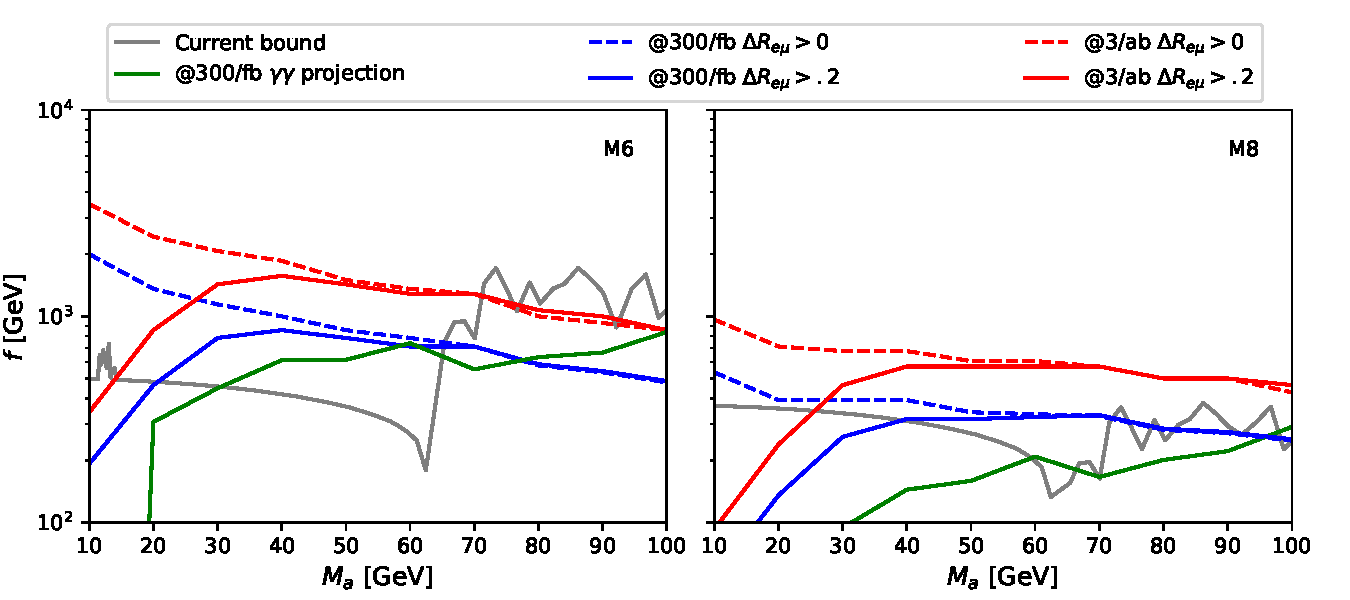
\includegraphics[width=0.99\textwidth]{\main/section7OtherSignatures/img/Fig2_TimidPNGB.pdf} 
\end{center}
\caption{\label{fig:Fig2TPNGB} Reach of the ditau search for the two
models M6 (left) and M8 (right), compared to the existing bounds (gray
lines). The existing bounds indicate the strongest exclusion amongst those
arising from dimuon searches~\cite{Chatrchyan:2012am}, diphoton searches~\cite{Aad:2014ioa,CMS:2017yta}, and BSM decay width
of the Higgs~\cite{Khachatryan:2016vau}. (The bounds from \citeref{Aaij:2017rft}, obtained adapting the analysis of \citeref{Haisch:2018kqx} to these models, turn out to be subleading.) We have also indicated the current bounds obtained by adapting the results in \citeref{Mariotti:2017vtv} for diphotons (green).
The projected reach is computed at 14 TeV using the HL-LHC detector simulation, for a luminosity of 300 (blue) and 3000 (red) $\text{fb}^{-1}$, and two distinct cuts on $\Delta R_{\mu e}$.}


\end{figure*}

A crucial discriminating variable in such search, particularly for the low mass region, is the angular separation $\Delta R_{e\mu}$ between the electron and the muon. We present the reach estimated from a cut-and-count simulation with the conservative choice $\Delta R_{e\mu}>0.2$ included or removed. In the plot we have not taken into account the systematic error in the background, but it is important to remark that, in order to take full advantage of the HL-LHC run, it should be kept below 2\%.\rt{Is this aligned with our recommendation for systematic uncertainties?} The additional cuts, discussed in \citeref{Cacciapaglia:2017iws}, are: $p_{T\mu}>50$~GeV, $p_{Te}>10$~GeV, $\Delta R_{\mu j}>0.5$, $\Delta R_{e j}>0.5$, $p_{Tj}>200$~GeV,  $\Delta R_{\mu e}<1$,  $m_{\mu e}<100$~GeV. Note that we also impose an upper bound on $\Delta R_{\mu e}$ to reduce the (mostly flat) $t \bar t$ background.

The heavier pseudo-scalar $\eta'$, not being a true Goldstone boson, could have a mass in the multi TeV range. Nevertheless, it may give observable signals at the LHC because it decays into final states such as $\gamma \gamma$, $Z\gamma$, $ZZ$, $WW$, $t\bar{t}$ and $Z h$ (the last one via top loops). In \fig{fig:Fig3TPNGB} we present the lower bounds on $f$ for the two models, in the $(M_a,\, M_{\eta'})$ mass plane. The white region corresponds to masses incompatible with the models~\cite{Belyaev:2016ftv}. 
The vertical band with a strong bound for $M_a \sim 215$~GeV corresponds to $Zh$ searches, which were not included in \citeref{Belyaev:2016ftv}. 

\begin{figure*}[t] 
\begin{center}
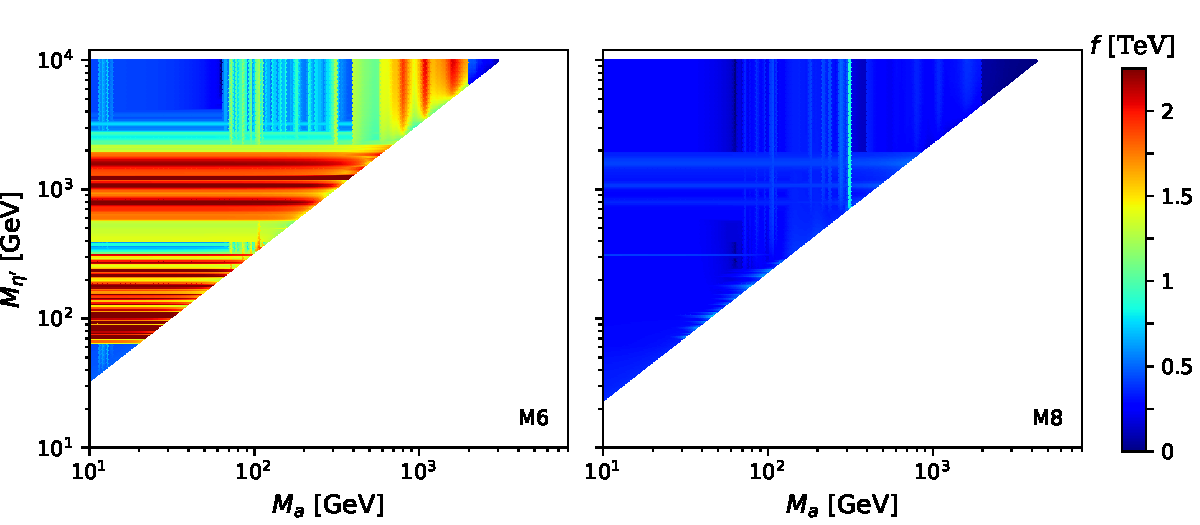
\includegraphics[width=0.99\textwidth]{\main/section7OtherSignatures/img/Fig3_TimidPNGB.pdf} 
\end{center}
\caption{\label{fig:Fig3TPNGB} Lower bound the Higgs decay constant $f$ for the two benchmark models M6 and M8 in the presence of both pseudo-scalars $a$ and $\eta'$.}
\end{figure*}


Figure~\ref{fig:Fig3TPNGB} takes into account the relevant searches performed with the 2016 data of about $36/\mbox{fb}$ of integrated luminosity at 13~TeV.
Similar analyses can of course be performed for the remaining models, but the two presented in this work are amongst the least constrained by current data.

In conclusion, the HL and HE phases of the LHC present us with newer possibilities to search for BSM physics. The models discussed here provide concrete examples where new physics could arise both in the high and low mass regime, benefiting from both improvements.

\textbf{Acknowledgments:} We wish to thank M. Selvaggi for help with the HL detector simulation in Delphes. Support: \textbf{G.C.:} Institut Franco-Suedois (project T{\"o}r) and  
the Labex-LIO (Lyon Institute of Origins) under grant ANR-10-LABX-66, FRAMA (FR3127,
F\'ed\'eration de Recherche ``Andr\'e Marie Amp\`ere''), \textbf{G.F.:} The Knut and Alice Wallenberg Foundation and the Lars Hierta Memorial Foundation \textbf{T.F.:} IBS under the project code, IBS-R018-D1, \textbf{H.S.:} ERC under the European Union's Horizon 2020 research and innovation programme (grant agreement No 668679).